 \begin{figure}[!ht]
	\begin{center}
		\makebox[\textwidth]{
			\centering
			\captionsetup{width=0.5\linewidth}
			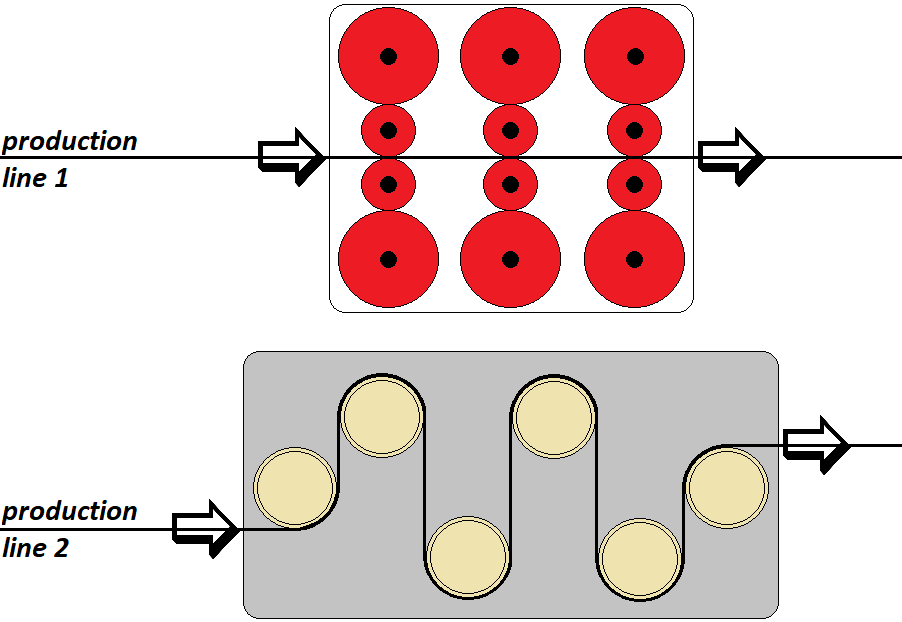
\includegraphics[width=0.9\linewidth]{../images/introduction-hypothetical_constraints.png}}
		\caption{Different Categories of Production Events Handling. The hot rolling mill positioned in production line 1 treats only one slab at a time. The unit in production line 2, pickling tank full of acid coloured in grey, treats the metal surface of more than one slab at a time.
		}
		\label{figure-hypothetical_constraints}
	\end{center}
\end{figure}